\documentclass[11pt,conference]{IEEEtran}

\usepackage[utf8]{inputenc}
\usepackage{hyperref}
\usepackage{graphicx}
\usepackage{wrapfig}

\begin{document}
\title{\huge Machine Learning Class Project 2 - Recommender System}

\author{
  Marta González, Natalie Bolón, Pau Argelaguet\\
  \small \textit{École Polytechnique Fédérale de Lausanne, Switzerland}
}

\maketitle

\thispagestyle{plain}
\pagestyle{plain}

\begin{abstract}
This project consists on applying machine learning techniques to predict user ratings on items. It is considered that those items are movies, but since no extra metadata is provided, they can be virtually anything. Not all users have rated all items, therefore, the system has to predict those unknowns using the given training data.
\end{abstract}

\section{Introduction}
The recommender system implemented in this paper is based on user feedback, that is, on ratings users leave on some items. The given dataset contains data about \verb|10000| users and \verb|1000| items, so an easy way to visualize this data would be by a matrix of \verb|10000| rows and \verb|1000| columns, where position \verb|M[i,j]| would be the rating (from 1 to 5) of the user \verb|i| to the item \verb|j|. Of course, not all users have rated all items -- in fact, quite the opposite: the vast majority of cells in the matrix are empty (represented by a 0), leading to a sparse matrix.

The main task of the project is to fill those 0 values into actual valid ratings between 1 to 5 that are as much similar as possible as what the user would hypothetically provide. For training the model, only the valid ratings are taken into account (i.e., those given in the train set between 1 and 5).

\section{Data preprocess}

There are two main goals in data preprocessing: getting the raw \verb|csv| data into a format understandable by the used tools and applying some feature engineering to get more relevant results from the training process.

The first step is quite straight-forward: the \verb|csv| file is parsed line by line into a pandas dataframe, that makes easier to do batch operations for preprocessing. Then, that dataframe is imported into the library-specific format that is optimized for the different algorithms to work. 

In terms of preprocessing, basically irrelevant users are discarded in order to make predictions, that is, given a threshold, users with less ratings than it are not taken in account when training the model (they not provide enough generalizable and reusable data for the rest of the model).

\textbf{Graphic diferent nombre minim numdata}

It's also worth mentioning that caching is implemented. Loading and processing big datasets is expensive, therefore that information is saved in \verb|pickle|-serialized objects. Trained models are saved automatically as well and can be loaded via a command line option\footnote{Check README.md for more information.}.

\section{Method selection}

The recommender system problem's aim is to discover a hidden structure in the ratings matrix so that it can generate the missing values with the minimum possible error. The rating matrix is characterized by being mainly sparse and diverse in the number of ratings per each user and ratings for each item. These 2 characteristics of the data strongly condition the choice of the model. The methods have been considered for this project have been:
\begin{itemize}
\item{Matrix factorization, with both stochastic gradient descent and alternating least squares}
\item{Neural Networks}
\item{Collaborative filtering}
\end{itemize}

These 3 methods apply to unsupervised learning and can be used for this type of datasets with missing entries. 

The first one, matrix factorization, is a matrix decomposition method which aim is to characterize items and users by matrices of  features inferred from the ratings matrix. This decomposition could be done by SVD but given the highly sparsity character of the matrix the results of this method are not accurate. Alternatively, applying non-negative matrix factorization leads to better results after correct tunning of hyper-parameters. NMF has been implemented using both stochastic gradient descent and coordinate descent (Alternating Least Squares) for updating both matrices. 

The second one, neural networks, has been implemented as a deep learning method to try to infer the underlying model in the ratings matrix. Even though the high potential of this method, it has not been considered as the principal possibility to approach the problem due to the character of the data. 

Finally, collaborative filtering is a method whose aim is to look for "similar" users and base the new rating on their previous ratings. Similarity of users can be expressed by giving to each pair of users a value concerning their distance. Many functions of distances can be used. This will be explored in the followings sections.

All these different methods will be evaluated with the same given loss function. In particular for this project, the loss function used is the mean squared error.

\section{Implementation}

\subsection{Matrix factorization}
The implementation of matrix factorization was done using an external library of Python called Surprise (see \cite{MF_Surprise}). This library computes non-negative matrix factorization using regularized stochastic gradient descent. Unlike other libraries such as SKlearn or Nimfa, Surprise supports matrix factorization for matrix reconstruction; i.e. for sparse matrices which results in a better prediction of the unknown values. Moreover, regularization terms has been introduced to avoid overfitting when increasing the number of features. Finally, the introduction of bias terms has been studied as a possible way to reduce the error but has been discarded after cross validation results showed higher error in the prediction when bias were used.
Finally, figure \ref{epochs} shows how the error decreases as the number of iterations increase. The decrease of the train error ensures the convergence of the method.
\begin{figure}[ht!]
	\centering
	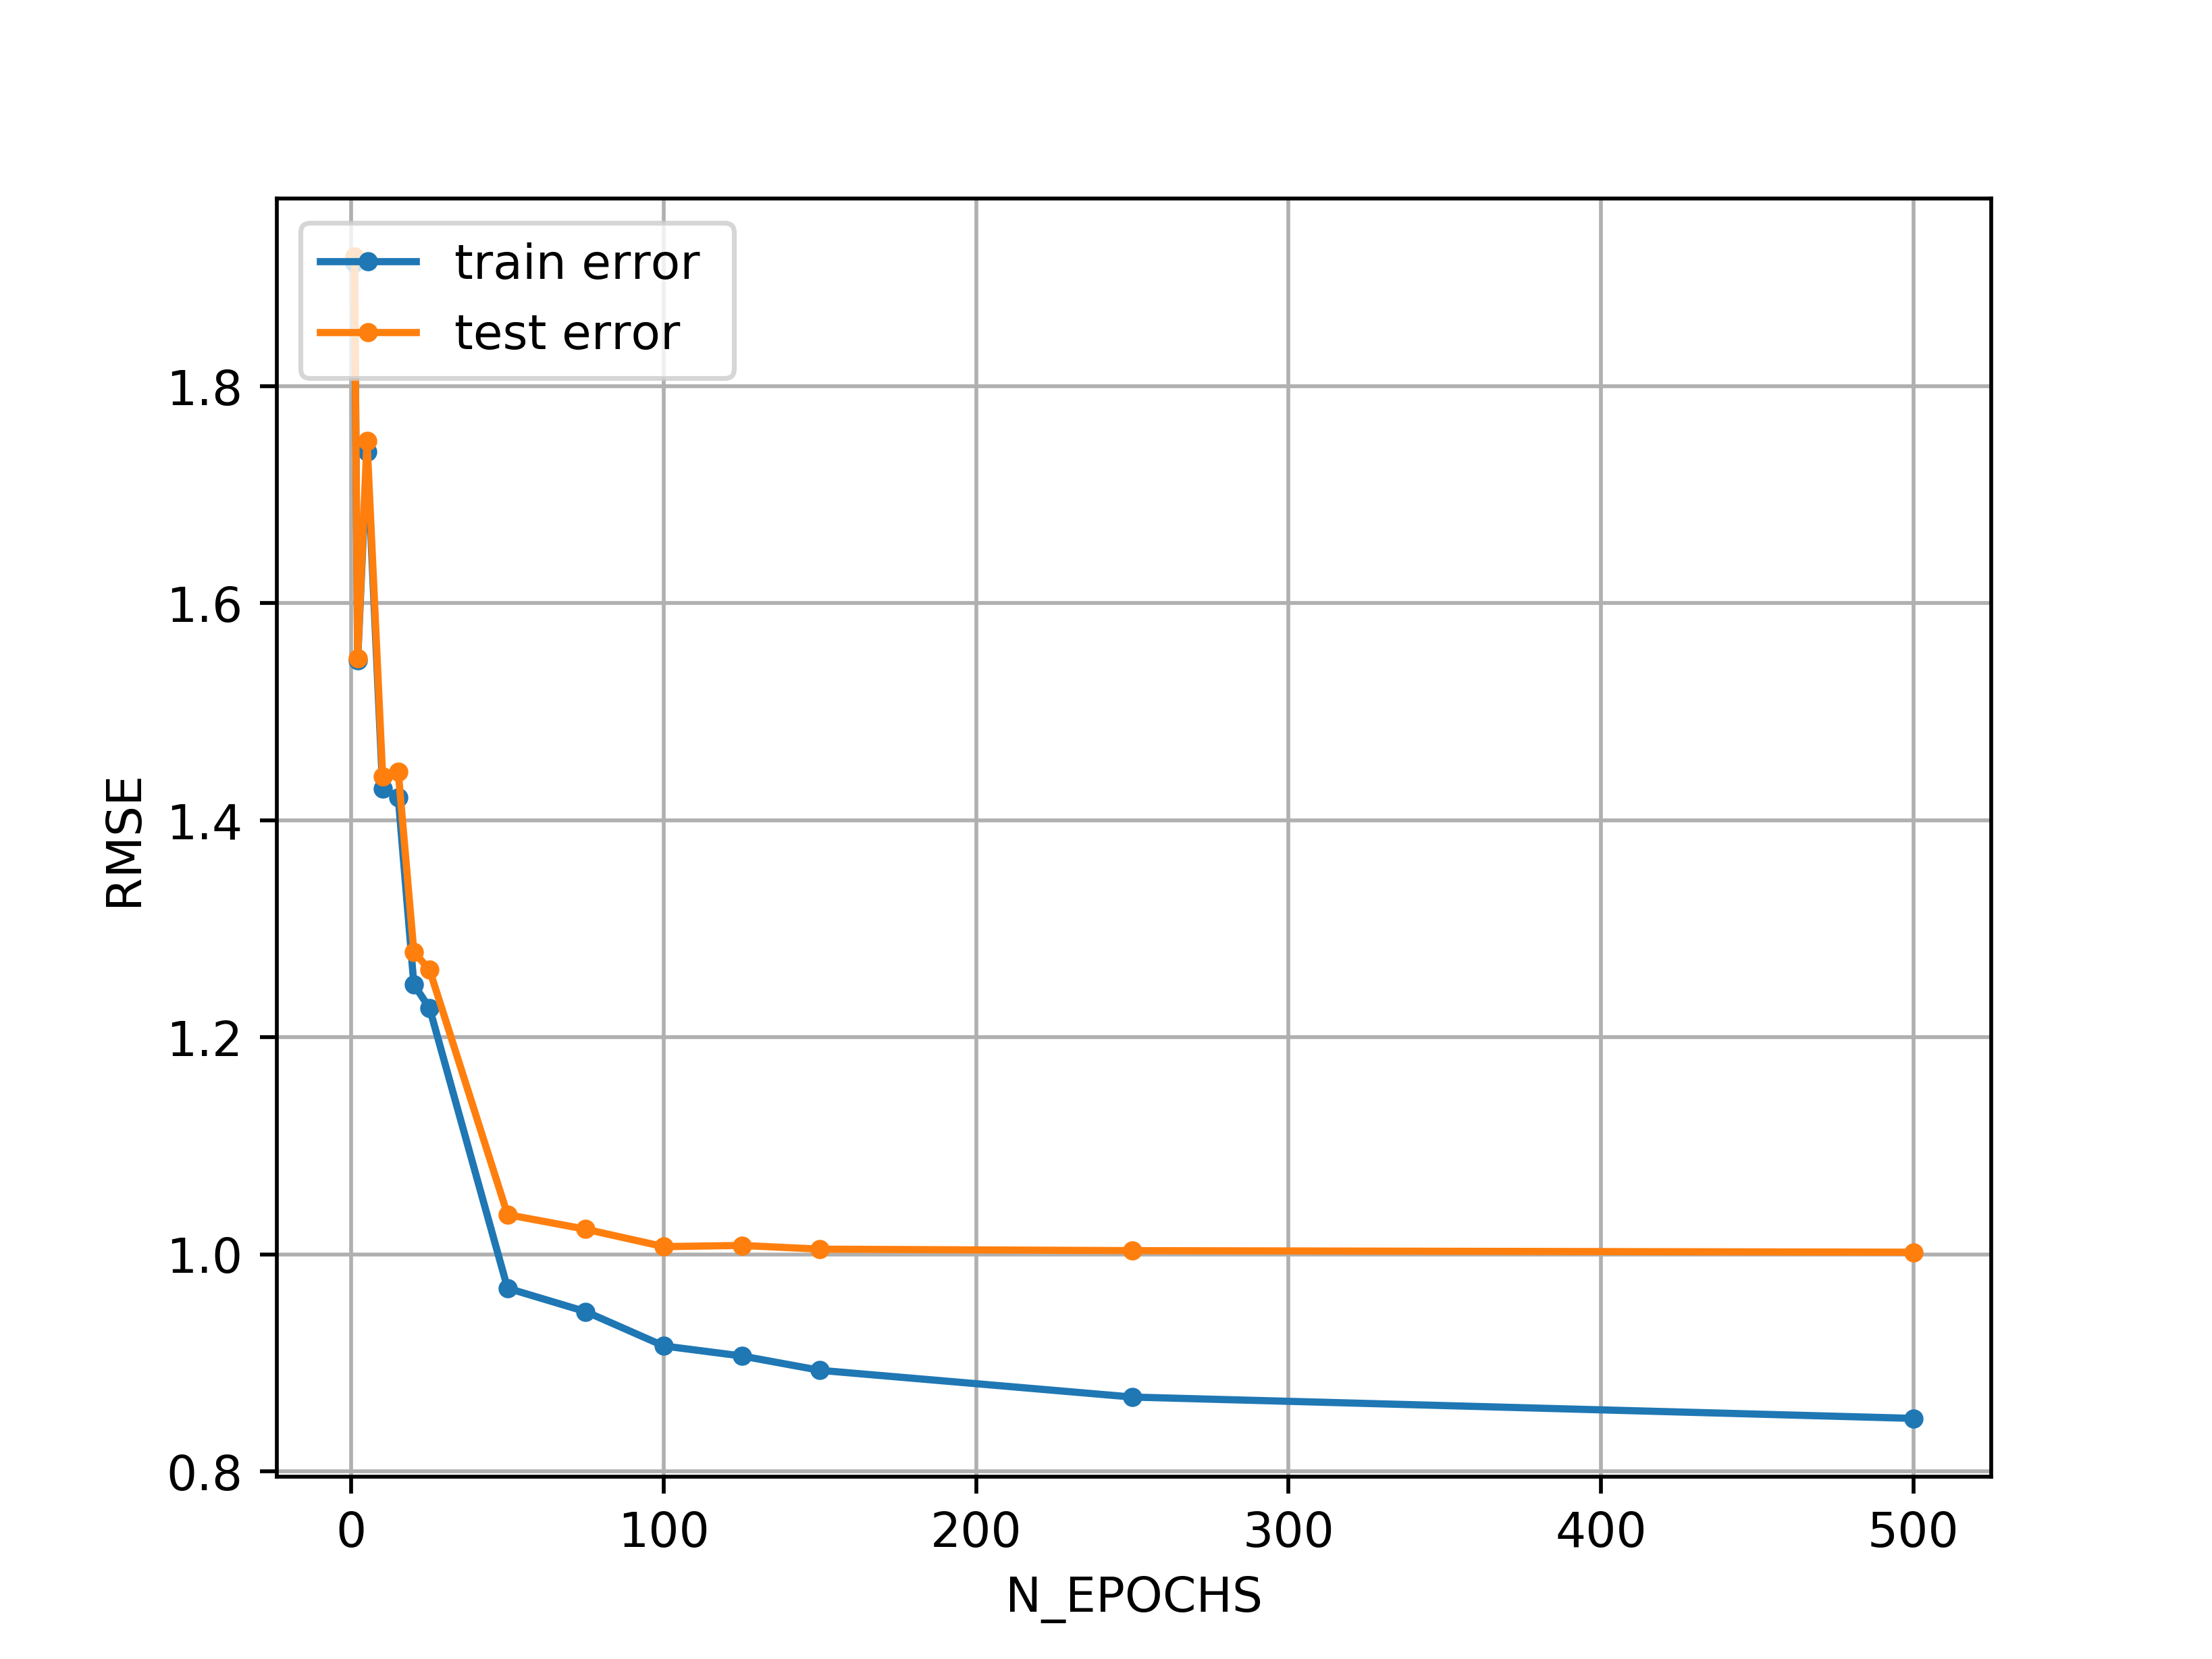
\includegraphics[width=265px]{RMSE_N_EPOCHS.png}
	\caption{RMSE for train and test data as the number of iterations increase}
    \label{epochs}
\end{figure}

\subsection{Neural Networks}
The implementation of a neural network has been done using Pytorch (see \cite{Pytorch}).  

\subsection{Collaborative filtering}  %Per si volem explicar coses del nostre collaborative filtering: Sklearn provides a package to compute those distances called pairwise.distance, and it includes many different distance functions.% 
Different distances for measuring similarities can be used in order to assign similarities between users. Surprise gives collaborative filtering algorithms and supports different distances. In particular in this project, KNNBaseline (see \cite{KNNBaseline}) has been considered with 3 distance functions: cosine, pearson$\_$baseline and MSD. The results for these distances are:
\\

\begin{table}[htbp]
\begin{center}
\begin{tabular}{|c|c|c|}
\hline
Pearson$\_$Baseline& Cosine & MSD \\
\hline 
0.9996 & 1.0128 & 1.0100  \\ \hline
\end{tabular}
\end{center}
\caption{RMSE for KNNBaseline and different distance functions}
\end{table}

\section{Hyperparameter tuning}
Each of the methods cited before consider different parameters such as the step size in matrix factorization using stochastic gradient descent or the number of layers in the model in the case of neural networks. To proceed with the tunning of hyperparameters for each method, 5-fold cross validation has been implemented and different range of values for each hyperparameter have been considered. 
\subsection{Matrix factorization}
NMF class from Suprise has several parameters to take into account such as the number of features in the factorization (n$\_$factors), the number of iterations (n$\_$epochs) or the regularization terms %els mirem?%.
It also accepts to add a bias term for user and item for each prediction. 
5-fold cross validation has been applied and it has yield to the following results:
The first thing to test is the use of the bias terms. The predictions can be made adding the value of the user bias and the item bias, and the following results have been recorded from values of n$\_$factors (number of features) from 15 to 30:

\begin{figure}[ht!]
	\centering
	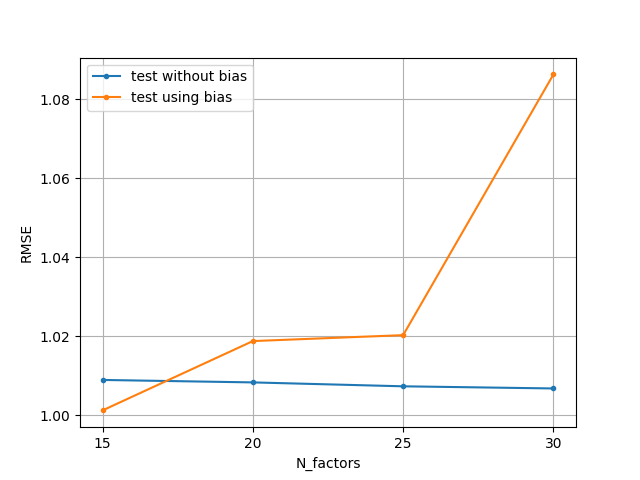
\includegraphics[width=265px]{Bias.png}
	\caption{Loss obtained by NMF applied to different number of features with and without bias terms, using 5-fold cross validation}
    \label{Bias}
\end{figure}

From figure \ref{Bias} it can be seen that the use of bias terms only give better results for low values of the number of features. This is due to the fact that bias terms are constant terms that are not learned, thus adding them only give best results in low-rank approximations. When increasing the rank, the model gets more complex and adding a constant term don't give lower errors. From now on then, bias terms will not be added to the predictions. 

Next hyperparameter to be tunned is the number of features to be considered in the factorization. Graphic number ... shows the RMSE value for different values of n$\_$factors. \textbf{Comprovar que si posem valors de nfactor molt grans error augmenta--> overfitting} 
\textbf{Graphic for diferent num of features}
To avoid overfitting, regularization terms can be add to the loss function. In this way, the minimization of the loss function implies that the norm of the matrices in the factorization will not be very large. Recall that the data matrix is factorized in two matrices, the first one known refers to the users and the second one to the items. In particular there will be two regularization terms, one for each matrix.

\begin{figure}[ht!]
	\centering
	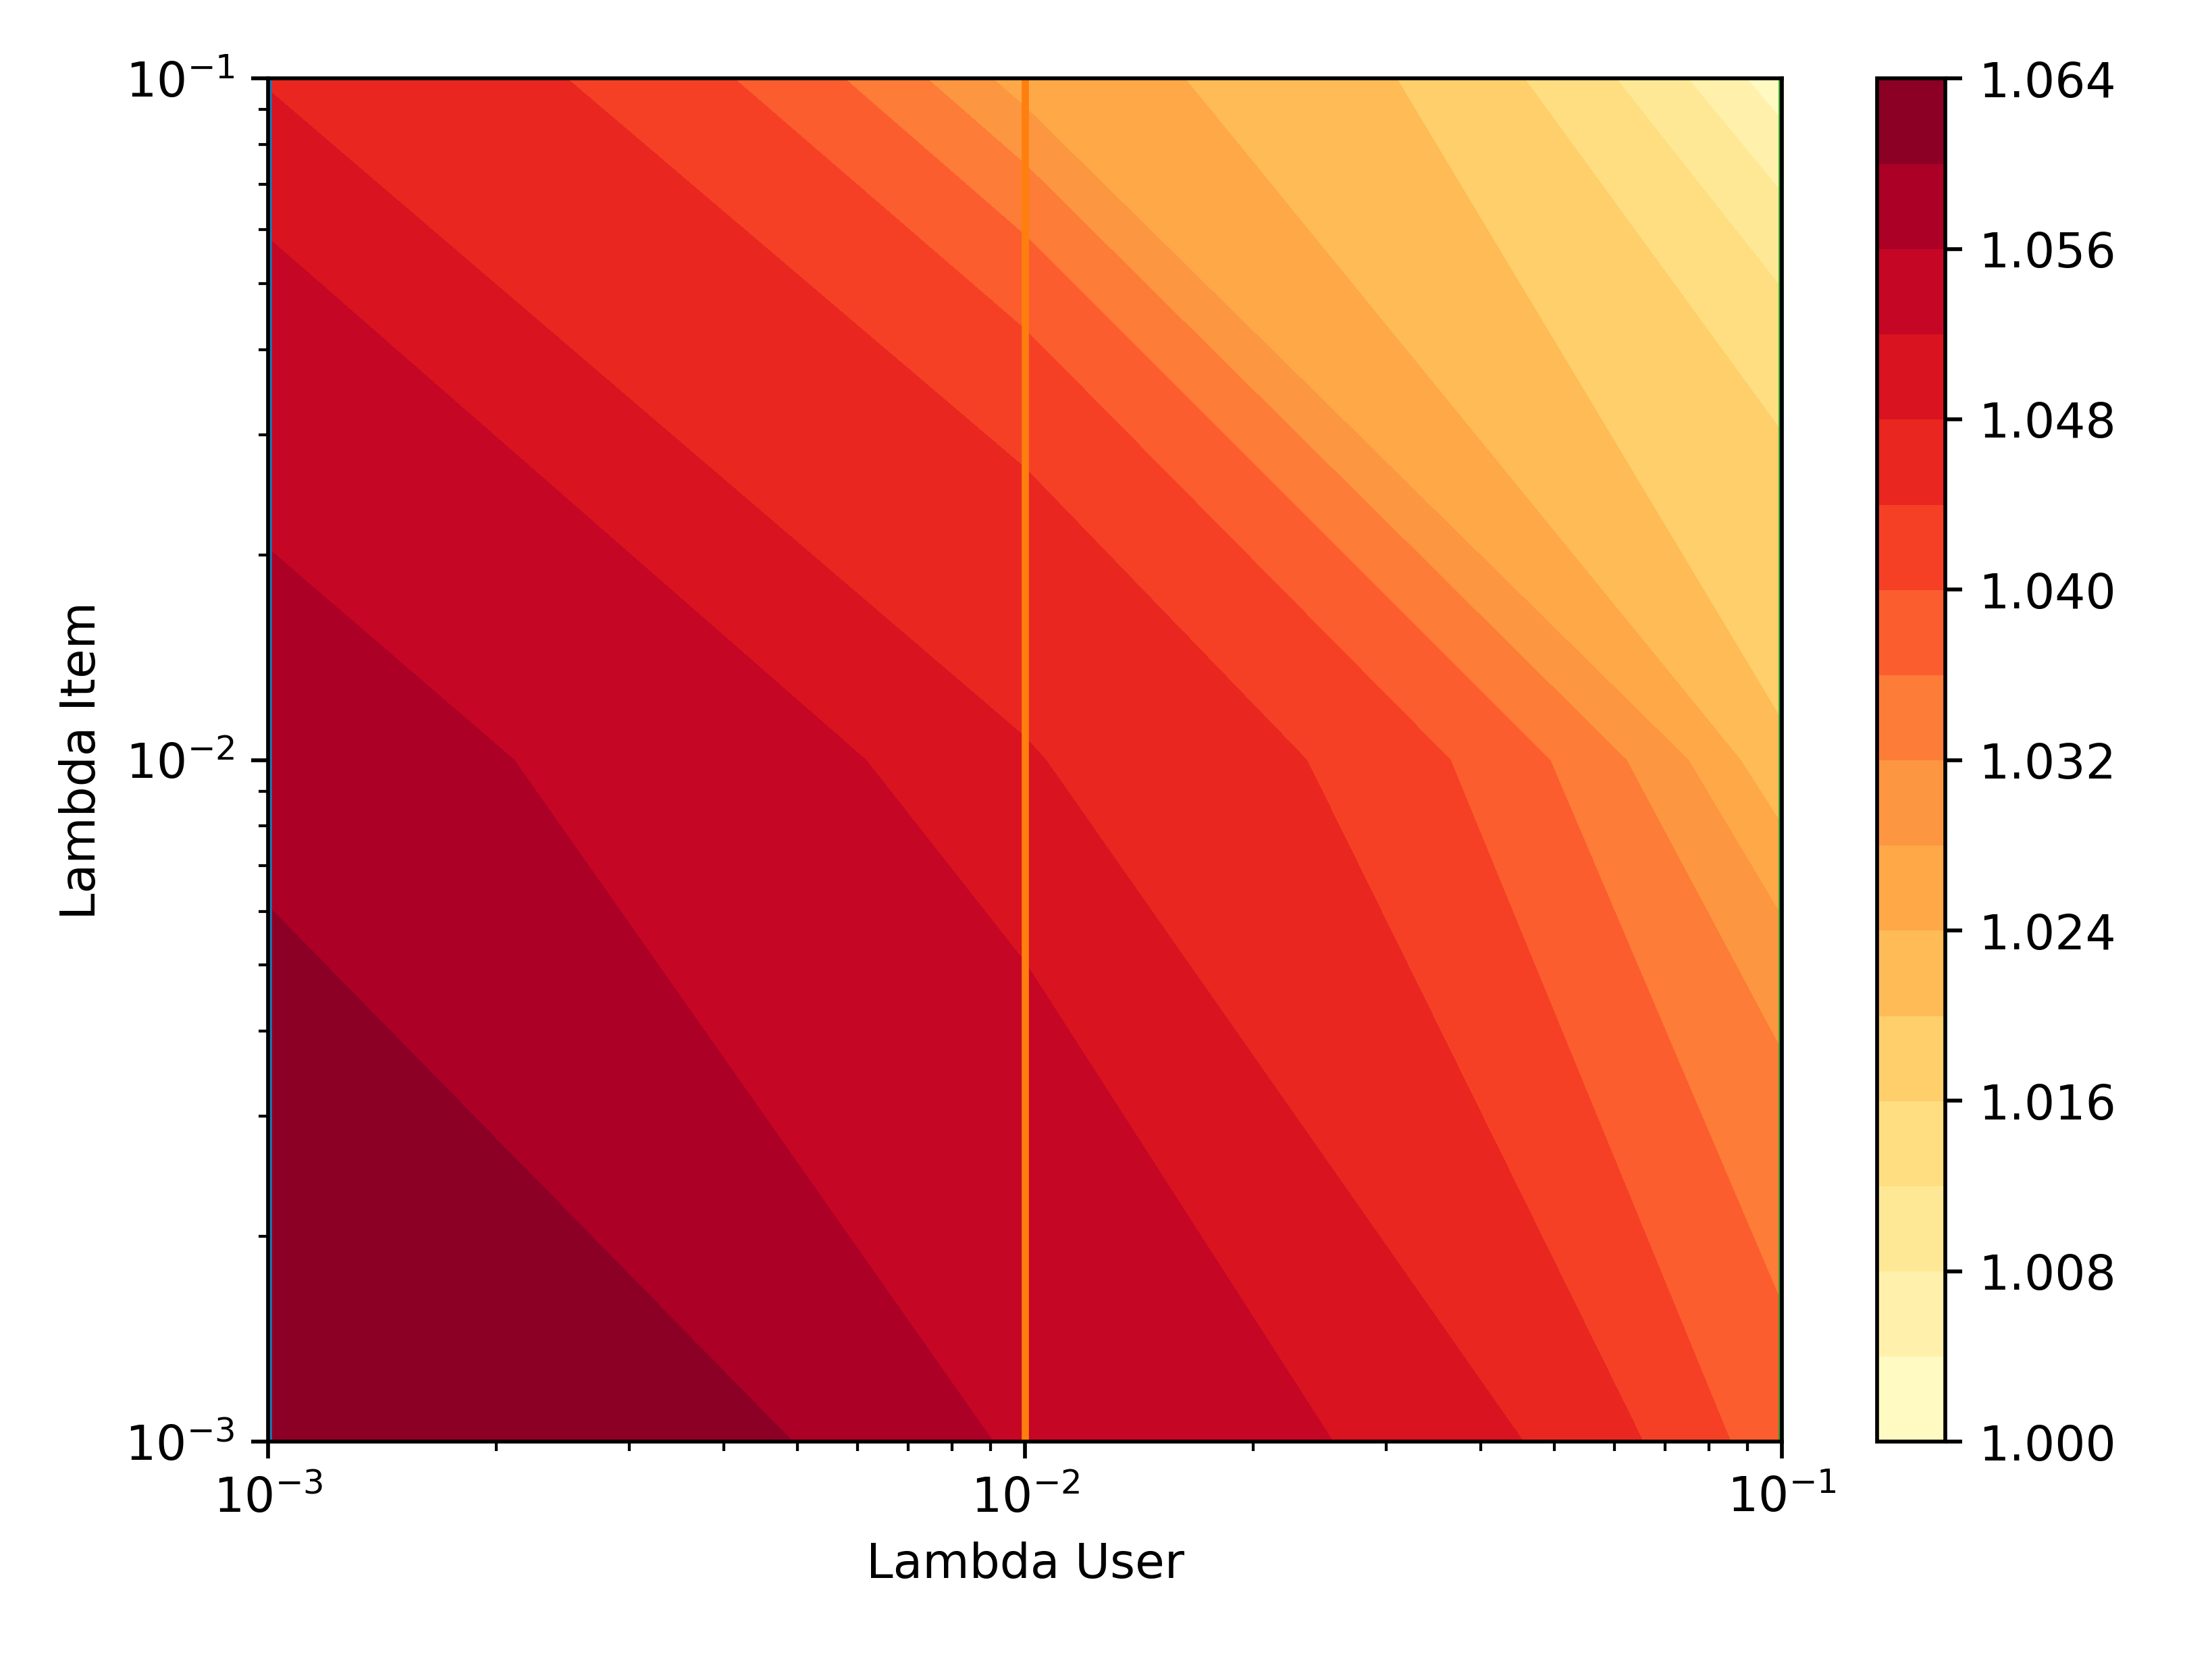
\includegraphics[width=265px]{lambdas.png}
	\caption{Loss obtained by NMF applied to different regularization terms using 5-fold cross-validation}
    \label{lambdas}
\end{figure}

In the figure \ref{lambdas} x-axis corresponds to the lambda of the user matrix and the y-axis to the lambda of the item matrix. The lowest RMSE is obtained using both lambdas equal to $10^{-1}$.

\subsection{Neural Networks}
A proof-of-concept has been implemented with a basic neural network structure. The hyperparameters tunned for this method have been the number of hidden layers and the size of this layers. Neither convolutional layers nor pooling have been considered. 

The best result have been achieved with three layers resulting in an rmse in the test set of 1.2447 which is far away from the best results obtained with other methods. 

Given the results obtained and based on previous research of methods applied for this problem (see \cite{Recommender Systems}), implementation of neural networks has been discarded as a possible way to improve the performance of the recommender system due to its complexity, high computational cost and variability in results. 


\subsection{Collaborative filtering}
The hyperparameters to tune in the collaborative filtering we have used, KNNBaseline, are basically 2; the maximum number of neighbors that takes into account in the prediction and the distance function considered. 

The first hyperparameter tunning is done in the maximum number of neighbors considered, named k in the function KNNBaseline. 

\begin{figure}[ht!]
	\centering
	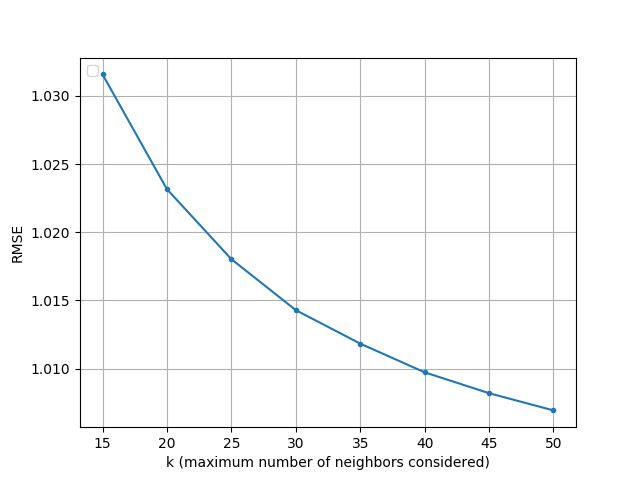
\includegraphics[width=265px]{k.png}
	\caption{Loss obtained by KNNBaseline applied to different k values using 5-fold cross-validation}
    \label{KNN1}
\end{figure}

The loss function decreases as the value k increases (figure \ref{KNN1}). Even though, if this value is very large it is necessary to save large amount of data in the similarity matrices, leading to high computational cost. As the error stabilizes around 45, higher values are not considered.

\section{Results and Summary}
After tunning all the hyperparameters, the best results for each method can be sumed up in the following table:
\begin{table}[htbp]
\begin{center}
\begin{tabular}{|c|c|c|} \hline
Method & Error & Parameters\\ \hline
Non-Negative Matrix factorization &  &Regularization terms = 0.1  \\
\hline 
Neural Network & 1.2447 &  \\ \hline
Collaborative filtering & 0.9996 & Distance function: Pearson$\_$Baseline \\ \hline
\end{tabular}
\end{center}
\caption{RMSE for KNNBaseline and different distance functions}
\end{table}
Comparing the errors applying the best hyperparameters, it can be seen that the lowest error is given by the non-negative matrix factorization method with ... features and regularization terms equal to 0.1.
The following best result is achieved by the collaborative filtering considering the Pearson correlation coefficient as the distance function (REPASSAR). And finally, neural networks didn't give such good results.

Matrix factorization and collaborative filtering are low-rank approximations of the original data matrix. The aim of these procedures is to explain the observations by a few underlying factors. In this project, our data consisted only in some ratings to films by some users, without any extra information about the user or the item. Thus, dimensionality reduction can provide useful results by creating new features.

Collaborative filtering can be implemented with many distance functions. In fact, one of the problems of a correct implementation is the correct choice of the distance function (reescriure).

Neural networks are complex and non-convex methods, and they are not specifically useful for recommender systems, where the data set does only give two features for each rating. MIRAR SI HI HA PAPERS QUE EXPLIQUIN QUE ES MES UTIL MATRIX FACTORIZATION.

Finally some problems arise in the resolution of this problem. Firstly, this is a non-convex optimization problem, which does not ensure the convergence to a global optimum, but local. And secondly, the dataset is strongly unbalanced and there are some users or/and items which do not have many items rated.

\begin{thebibliography}{9}
\bibitem{MF_Surprise}
Surprise - Python Scikit \url{http://surprise.readthedocs.io/}
\bibitem{Pytorch}
Pytorch Neural Networks \url{http://pytorch.org/}
\bibitem{KNNBaseline}
KNNBaseline\url{http://surprise.readthedocs.io/en/stable/knn_inspired.html}
\bibitem{Recommender Systems}
Recommender Systems\url{http://www.csc.kth.se/~miksa/papers/AutomaticMovieRatingsPrediction_MIPRO.pdf}
\end{thebibliography}

\end{document}
